\documentclass[11pt]{article}
%\documentclass[11pt]{report}
\usepackage{amsmath}
\usepackage{amsfonts}
\usepackage{amssymb}
\usepackage{graphicx} %perch� mi d� prob nella compilazione
%\usepackage{booktabs}
\usepackage{color}
\usepackage[applemac]{inputenc}
\usepackage[english]{babel}
%\usepackage{cancel}
%\usepackage{dsfont}
%\usepackage{hyperref}

\def\red{\color{red}}
\def\black{\color{black}}
\def\blue{\color{blue}}
\def\green{\color{green}}
\def\gray{\color{gray}}
\def\cyan{\color{cyan}}
\def\magenta{\color{magenta}}
\def\yellow{\color{yellow}}
\def\violet{\color{violet}}
\def\yellow{\color{yellow}}

%\def\blue{\color{blue!80!cyan}}

% \def\blue{\color{blue}}
 \def\cre{\color{red}}
 \def\cbl{\color{black}}
\definecolor{eublue}{rgb}{0.1,0.1,0.5} % Definition of blue color
\definecolor{eumagenta}{rgb}{1,0,0.9} % Definition of blue color


\setlength{\textwidth}{16.5cm} \setlength{\textheight}{24cm}
\setlength{\oddsidemargin}{-0cm}
\setlength{\evensidemargin}{-0.5cm} \setlength{\topmargin}{-2cm}
\renewcommand{\baselinestretch}{1.3}
\newcommand{\ud}{\mathrm{d}}


%%% stuff for theorem-like environments
\newtheorem{definition}{D�finition}
\newtheorem{theorem}{Th�or�me}
\newtheorem{lemma}{Lemme}
\newtheorem{remark}{Remarque}
\newtheorem{proposition}{Proposition}
\newtheorem{corollary}{Corollaire}
\newcommand{\bpf}{{\bf Preuve }}
\newcommand{\epf}{\begin{flushright}$\blacksquare$\end{flushright}}


\newcommand{\BE}{\begin{equation}}
\newcommand{\BEno}{\begin{equation*}}
\newcommand{\EE}{\end{equation}}
\newcommand{\EEno}{\end{equation*}}
\newcommand{\mtx}[1]{\left[\begin{matrix}#1\end{matrix}\right]}

%%% probability symbolism
%\newcommand{\operatorname}{\mathop}
\newcommand{\logit}[1]{\operatorname{logit}\left(#1\right)}
\newcommand{\prob}[1]{\operatorname{\mathbb P}(#1)}
\newcommand{\probstar}[1]{\operatorname{P}^*(#1)}
\newcommand{\expect}[1]{\operatorname{\mathbb E}\left[#1\right]}
\newcommand{\expectsub}[2]{\expectation_{#1}\left(#2\right)}
\newcommand{\variance}[1]{\operatorname{Var}\left(#1\right)}
\newcommand{\covariance}[2]{\operatorname{Cov}\left(#1,#2\right)}
\newcommand{\correlation}[2]{\operatorname{Corr}\left(#1,#2\right)}
\newcommand{\normaldensity}[3] {\frac1{\sqrt{2\pi#3}}\exp\left[-\frac1{2#3} (#1-#2)^2\right]}

\newcommand{\trace}[1]{\operatorname{trace}\left(#1\right)}

\newcommand{\iid}{\stackrel{\mathrm{iid}}{\sim}}
\newcommand{\app}{\stackrel{\mathrm{app}}{=}}
%%% different fields in mathematics
\newcommand{\naturals}{\mathbb{N}}
\newcommand{\reals}{\mathbb{R}}
\newcommand{\posreals}{\reals_+}
\newcommand{\realvectors}[1]{\reals^{#1}}
\newcommand{\complex}{\mathbb{C}}
\newcommand{\integers}{\mathbb{Z}}

\newcommand{\mT}{\mathcal{T}}
\newcommand{\mF}{\mathcal{F}}
\newcommand{\mS}{\mathcal{S}}
\newcommand{\mN}{\mathcal{N}}
\newcommand{\mP}{\mathcal{P}}
\newcommand{\mC}{\mathcal{C}}
\newcommand{\mU}{\mathcal{U}}
\newcommand{\mR}{\mathcal{R}}

\newcommand{\bzero}{\text{\mathversion{bold}$0$\mathversion{normal}}}
\newcommand{\buno}{\text{\mathversion{bold}$1$\mathversion{normal}}}
%%% and greek
\newcommand{\bSigma}{\text{\mathversion{bold}$\Sigma$\mathversion{normal}}}
\newcommand{\bmu}{\text{\mathversion{bold}$\mu$\mathversion{normal}}}
\newcommand{\bnu}{\text{\mathversion{bold}$\nu$\mathversion{normal}}}
\newcommand{\btheta}{\text{\mathversion{bold}$\theta$\mathversion{normal}}}
\newcommand{\brho}{\text{\mathversion{bold}$\rho$\mathversion{normal}}}
\newcommand{\balpha}{\text{\mathversion{bold}$\alpha$\mathversion{normal}}}
\newcommand{\bbeta}{\text{\mathversion{bold}$\beta$\mathversion{normal}}}
\newcommand{\bGamma}{\text{\mathversion{bold}$\Gamma$\mathversion{normal}}}
\newcommand{\bLambda}{\text{\mathversion{bold}$\Lambda$\mathversion{normal}}}
\newcommand{\blambda}{\text{\mathversion{bold}$\lambda$\mathversion{normal}}}
\newcommand{\bdelta}{\text{\mathversion{bold}$\delta$\mathversion{normal}}}

\newcommand{\veps}{\varepsilon}
\newcommand{\vphi}{\varphi}
\newcommand{\bra}[1]{\{#1\}}
\newcommand{\indic}{\mathds{1}}

\begin{document}
\noindent
\begin{center}

\includegraphics[width=2.5cm]{logo}\\
\vspace{1cm}
{\huge{\bf{Balancing of Food Balance Sheets (FBSs)}}}   \\
\bigskip
{\large {\bf Marco Garieri, Natalia Golini, Luca Pozzi}} \\
{\large {\bf [name.cognome]@fao.org}} \\
{\large {\today}} \\
\end{center}
\tableofcontents



\section*{Abstract}
The balancing of FBSs represents a priority goal of FAO because they provide the main source of information for assessing world food situation and in order to establish the statistical base of FAO's plans for agricultural development. In this work we present a first attempt to solve the problem of balancing of FBSs. Taking advantage of the methodology developed in the statistical literature for a problem called ``sampling contingency tables'', we propose a version of the methodology that is suitable to the type of data we have available. 
%Initial results from a small simulation study (section 3) are encouraging, and then will look for improvements in this direction.

%In the previous years a proper working methodology was not proposed and for this reason a new approach has been developed. Bla bla bla...

%The balancing of Food Balance Sheets\\
%\black{Questions:}
%\begin{itemize}
%\item What is a food balance sheet?
%\item Why and when a food balance sheet is unbalanced?
%\item How to solve this problem?
%\end{itemize}


\newpage
\section{Problem Description}
This paper describes the details of novel methodology for balancing FAO Food Balance Sheets (FBSs). A FBS represents a comprehensive picture of the pattern of a country's food supply during a specific reference period. The FBS contains information on the sources of supply and its utilization for each food item i.e. each primary commodity available for human consumption.\\
The sources of supply are of three different kinds: production, imports and stock at the beginning of the reference period. For the utilization several entities define the formulation: food, seed, feed, industrial use, losses, exports and stock at the end of reference period. 
As stated above Total Supply (TS)  and Total Utilization (TU) are defined for each food item ($i$) in a given country ($c$) during the period ($t$) as follows:
$$ TS_{i,c,t} =Production_{i,c,t} +Imports_{i,c,t}+ Stock_{i,c,t-1} $$
\begin{eqnarray*}
TU_{i,c,t} &=& Food_{i,c,t} + Seed_{i,c,t} + Feed_{i,c,t} + IndUse_{i,c,t} \\
\nonumber &+& OtherUse_{i,c,t} + Losses_{i,c,t} + Exports_{i,c,t}\\
\nonumber &+&  Stock_{i,c,t}
\end{eqnarray*}
\noindent
In order to have a ``closed'' FBS, for each item (or commodity) the sources of supply need to be equal to its utilization for a given country during a particular year. Written in mathematical terms, the following equation needs to hold:
\begin{eqnarray}
TS_{i,c,t}=TU_{i,c,t} \quad \forall i
\label{bil}
\end{eqnarray}
The main problem is that a FBS is assembled from a variety of different sources, both official and unofficial. For this reason we rearrange the balancing equation in \ref{bil} placing to the left of the equation the terms that come from official sources (hereafter called consolidated terms) and placing to right those that come from unofficial sources. Note that the consolidated terms may change from country to country.
Thus, the aim of the project becomes the estimation the Supply Utilization Accounts (SUA) for a particular country, at a particular time for all the commodities, which are not consolidated.

\subsection{Toy Example}
%In the following table the first lines of the Italian FBS for 2009 is showed. In particular the ``consolidated'' columns are marked in orange, thus the values that are assumed as fixed.
%\begin{center} 
%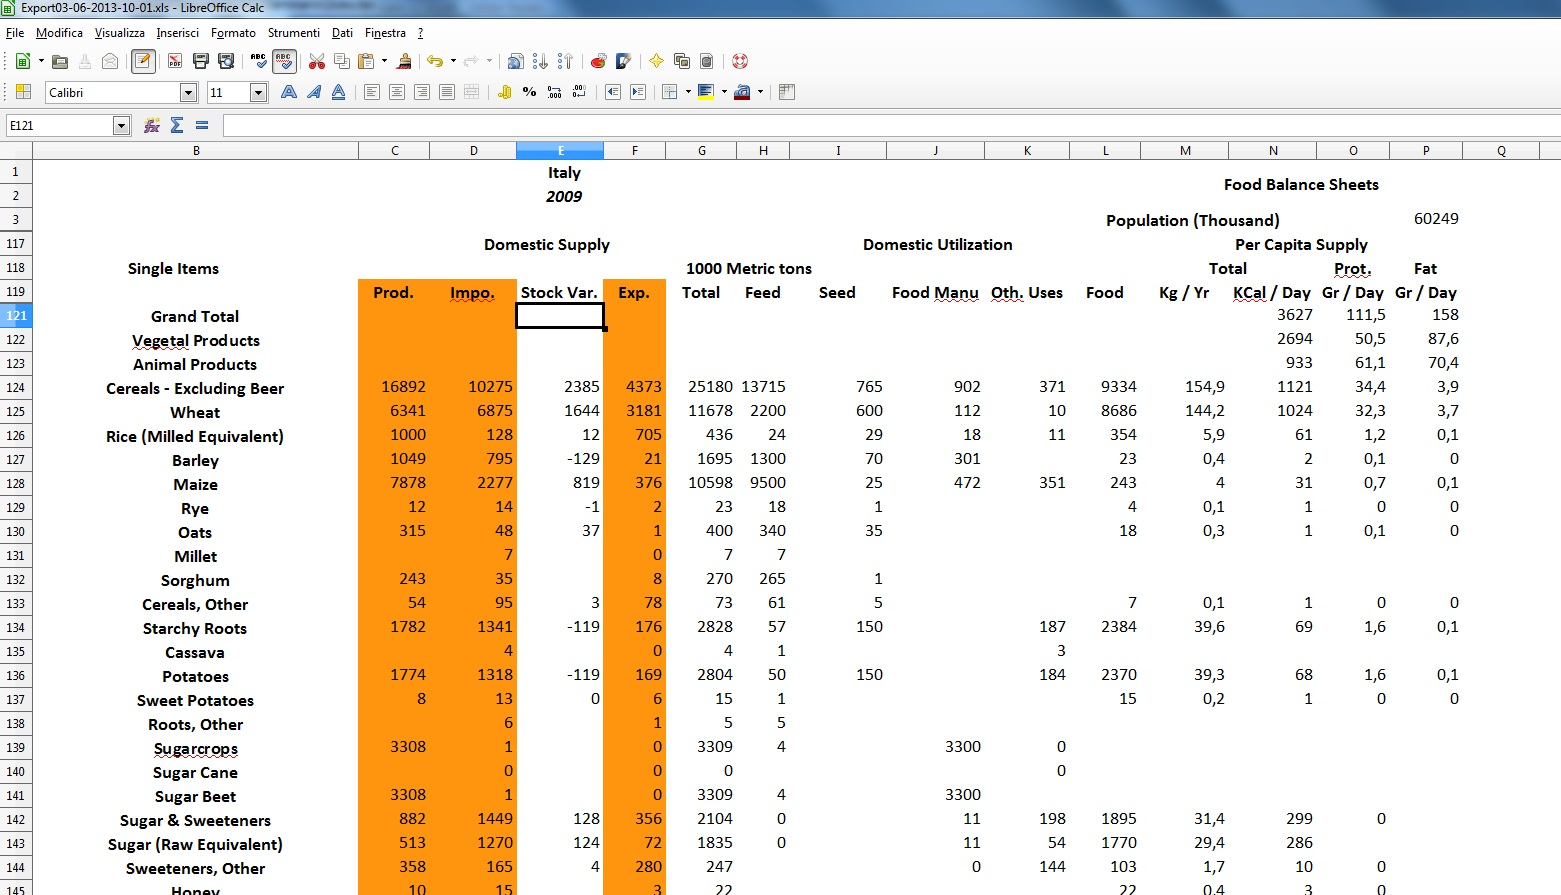
\includegraphics[scale=0.40]{Tab.jpg}
%\end{center}


In Table 1 we show the an example of FBS for a particular country at a particular year (i.e. Italy 2009). Here we assume that the consolidated terms are the production, imports and exports. Then we rearrange the balancing equation in order to have of the left side of equation the consolidated terms and the others on the right side, as in the following formula:

\begin{eqnarray}{\nonumber}
Production_{i,c,t}+ Imports_{i,c,t}-Exports_{i,c,t}  &=&  Food_{i,c,t} + Seed_{i,c,t} + Feed_{i,c,t}\\ 
\nonumber &+& IndUse_{i,c,t} + OtherUse_{i,c,t} \\
\nonumber &+& Losses_{i,c,t} -  StockVar_{i,c,t}
\end{eqnarray}
where $StockVar$ represents the changes in stocks occurring during the reference period. And with the assumption that it can assume both positive or negative values.



\black{
\begin{table}
\center
\label{Table 1}
    \begin{tabular}{ |l|c|c|c|c|c|c|c|r|}
    \hline
    Item & Food & Feed & Seed & IndUse & OthUse & StVar  & Tot \\ \hline \hline
    Cereals & 9334 & 13715 & 765 & 902 & 371 &  2385 &  22702 \\ \hline 
    Wheat	& 8686 & 2200  & 600 & 112 & 10 & 1644 & 9964 \\ \hline 
    Rice	& 354 & 24 & 29 & 18 & 11 & 12 & 424 \\ \hline
    \ldots	& \ldots & \ldots & \ldots & \ldots & \ldots & \ldots & \ldots \\ \hline
    .. \ldots & \ldots & \ldots & \ldots & \ldots & \ldots & \ldots & \ldots \\ \hline
    Oats & 18 & 340 & 35 &  &  & 37 & 356  \\ \hline          
    .. \ldots & \ldots & \ldots & \ldots & \ldots & \ldots & \ldots & \ldots \\ \hline
    Potatoes  & 2370 & 50 & 150 & & 184 & -119 & 2873 \\ \hline
    Sweet Pot. & 15 & 1 & & & & 0 & 16 \\ \hline
%    .. \ldots & \ldots & \ldots & \ldots & \ldots & \ldots & \ldots & \ldots \\ \hline
    \ldots & \ldots & \ldots & \ldots & \ldots & \ldots & \ldots & \ldots \\ \hline
   % Tot & 110203 & 30772 & 1981 & 34294 & 6104 & 5636 & 183329 \\ \hline            
    \end{tabular}
    \caption{FBS of Italy in 2009}
\end{table}


\noindent Each line represents a different commodity. The last column (Tot) is the total of the previous columns given the following formula:
$$ \text{Tot = Food + Feed + Seed + IndUse + OthUse - StVar}$$
In the Table \ref{Table 2} an additional column (Tot2) is added. Tot2 is described by the following formula:
$$ \text{Tot2 = Production + Imports - Exports} $$
Tot2 thus represents the trusted ``consolidated term''. A discrepancy occurs with the two different totals (Tot and Tot2) which leads to a non-closed FBS.\\
If and only if, for each line of the table, Tot = Tot2, the FBS has a closed form, and can be called Food \underline{Balanced} Sheet.\\\\
Three additional information can help in order to solve the problem:
\begin{itemize}
\item A prior information on the possible value of the cells. The information for each cell is given in a  distribution form (the details on that will be given in the next section)\footnote{Several groups within FAO-ESS are working in specific estimate problems for Food, Feed, Seed, Losses, etc.}
\item Some cells are \underline{structural zeros}, which means they are zero and they cannot take any other possible value
\item An estimate of the interval where the totals of the different columns should fall into
\end{itemize}


\vspace{0.5cm}
\begin{table}
\caption{FBS of Italy in 2009}
\center
\label{Table 2}
    \begin{tabular}{ |l|c|c|c|c|c|c|c|c|r|}
    \hline
    Item & Food & Feed & Seed & IndUse & OtherUse & StVar  & Tot & Tot2\\ \hline \hline    
    Cereals & 9334 & 13715 & 765 & 902 & 371 &  2385 &  22702 & 22794\\ \hline 
    Wheat	& 8686 & 2200  & 600 & 112 & 10 & 1644 & 9964 & 10035 \\ \hline 
    Rice	& 354 & 24 & 29 & 18 & 11 & 12 & 424 & 423\\ \hline
    \ldots	& \ldots & \ldots & \ldots & \ldots & \ldots & \ldots & \ldots & \ldots \\ \hline
    .. \ldots & \ldots & \ldots & \ldots & \ldots & \ldots & \ldots & \ldots & \ldots \\ \hline
    Oats & 18 & 340 & 35 &  &  & 37 & 356 & 362 \\ \hline          
    .. \ldots & \ldots & \ldots & \ldots & \ldots & \ldots & \ldots & \ldots & \ldots \\ \hline   
    Potat.  & 2370 & 50 & 150 & & 184 & -119 & 2873 & 2947\\ \hline
    Sweet Pot. & 15 & 1 & & & & 0 & 16 & 15 \\ \hline
%    .. \ldots & \ldots & \ldots & \ldots & \ldots & \ldots & \ldots & \ldots & \ldots \\ \hline
    \ldots & \ldots & \ldots & \ldots & \ldots & \ldots & \ldots & \ldots & \ldots \\ \hline
%   Tot. & 110203 & 30772 & 1981 & 34294 & 6104 & 5636  & 177718 & 183329\\ \hline
    \end{tabular}
\end{table}
\vspace{6cm}
%Marginal-only contest \& Balancing problem\\
%\begin{itemize}
%\item \blue{Marginal-only contest}
%	\begin{itemize}
%		\item The full cell counts $n_{ij}$ are \underline{unrecorded}
%		\item Only the row and column totals are observed
%	\end{itemize}
%\yellow{Current application areas:} \black{genetics, medicine, social sciences and census data}. Here, data are released in the form of \yellow{marginal totals} \\
%\black{Distribution of a contingency table conditioned on summarized values of cell counts is a key to measuring the uncertainty for a table in traditional inference}
%\vspace{0.5cm}
%\item \blue{Balancing problem}:
%	\begin{itemize}
%		\item Since the full cell values are \underline{recorded with error} are considered as \emph{missing data}
%		\item The row and column totals are observed
%		%\item however the values ​​assumed by the cells can be positive or negative for StockVar.
%		\item The values assumed by the cells can be positive or negative for ``StockVar''
%	\end{itemize}
%\end{itemize}

%}

\section{Methodology}
\subsection{Theory}
Due to the lack of strong constraints (the only one available is the total of the rows), we decided to chose a strategy able to find a solution row by row (commodity by commodity) and in the last step a validation of the results is applied on the total of the columns.\\
Let us assume we fix a particular country and a particular year, the procedure will be the same for different countries and different years. Then we have a table, where for each row there is a commodity C, and for each column we have the different levels L (Food, Feed, Seed, Losses, StVar, IndUse and OtherUse).
For each commodity C, the only fixed value is the total of the row R, given by official information (e.g. this value is calculated as Production+Imports-Exports)
\vspace{0.5cm}
\begin{center}
    \begin{tabular}{ |c|c|c|c|c|c|c|c|}
    \hline
		& $L_1$ & $L_2$ & \ldots & $L_j$ & \ldots & $L_s$ & Tot\_rows \\ \hline
	$C_1$ & $x_{11}$ & $x_{12}$ & \ldots & $x_{1j}$ & \ldots & $x_{1s}$ & $R_{1}$ \\ \hline
		$C_2$ & $x_{21}$ & $x_{22}$ & \ldots & $x_{2j}$ & \ldots & $x_{2s}$ & $R_{2}$ \\ \hline
		\ldots & \ldots & \ldots &  \ldots & \ldots & \ldots & \ldots & \ldots \\ \hline
		$C_i$ & $x_{i1}$ & $x_{i2}$ & \ldots & $x_{ij}$ & \ldots & $x_{is}$ & $R_{i}$ \\ \hline		
		\ldots & \ldots & \ldots &  \ldots & \ldots & \ldots & \ldots & \ldots \\ \hline		
		$C_r$ & $x_{r1}$ & $x_{r2}$ & \ldots & $x_{rj}$ & \ldots & $x_{rs}$ & $R_{r}$ \\ \hline
Tot\_cols & $T_{1}$ & $T_{2}$ & \ldots & $T_{j}$ & \ldots & $T_{s}$ & \\
\hline		
	\end{tabular}
\end{center}
\vspace{0.5cm}
\noindent
{\bf Prior information:}
\begin{itemize}
\item The totals of the rows $R_i$, given as fixed number
\item The distribution of the different cells with are not structural zero $x_{ij}\sim\mT\mN(\mu_{ij}, \sigma^2_{ij})$, where $\mu_{ij}$ is the estimated mean and a fixed standard deviation $\sigma_{ij}$ with bounds given as a prior information.
The shape of the distribution will change dependently with the prior information we have for that particular commodity C in that particular level L. We know since the beginning that the estimates of particular levels L are more accurate than others, then if it is more accurate it will be closer to a normal distribution, otherwise it will be like a uniform distribution within the bounds
\item The range of the possible outcomes of the columns' totals $T_j$, given as interval ($t_{j,min}$, $t_{j,max})$
\end{itemize}
Working independently row by row, we sample cell by cell from the given distribution until the last value of the row which will be given as difference from the total of the row $R$ and the sum of all the previous sampled values (this value needs to fall within the given distribution for that cell, and thus a control for this is implemented). If we are successful with all the cells, the column's totals $T$ are calculated. The table is acceptable if for all the columns, the observed value of $T$ falls inside the given interval $(t_{j,min}$, $t_{j,max})$, otherwise we reject the table and start again.

\subsection{Algorithm}
\begin{enumerate}
\item For each row $R_i$ (say commodity) of length $s$:
\begin{enumerate}
\item Set the last cell of the row $x_{is}$ as StockVar, otherwise as the one with the biggest bounds
%\item For each row of length $s$ sample all cell beside the last one ($x_s$)
\item Sample all cells beside the last one, $x_{is}$
\item Compute $x_{is}$ as difference from the totals minus all previous values: $x_{is} = R_i-\sum_{j=1:s-1}x_{ij}$
%\item The last cell is calculated as: $x_{s} = R-\sum_{j=1:s-1}x_{j}$
%\item Check if $x_{is}$ falls inside $x_{is}\sim\mN(\mu_{s}, \sigma^2_{s})$, if not, sample again from the first cell of the row
\item Check if $x_{is}$ falls inside $x_{is}\sim\mT\mN(\mu_{is}, \sigma^2_{is})$, if not, sample again from the first cell of the row
\end{enumerate}
\item Once all rows $R_i$ are sampled:
\begin{enumerate}
%\item Once all rows are sampled, calculate all the columns total $T$
\item Compute the column totals $T_j$
\item Check for all if $T_j$, $t_{j,min}\le T_j\le t_{j,max}$ is respected
\begin{itemize}
\item If previous step succeed, the table is accepted as a solution
\item If previous step did not succeed, the algorithm starts from the beginning
\end{itemize}
\end{enumerate}
\end{enumerate}

%\section{Simulation on sample table}\label{sez}
%The first algorithm has been tested for a simple example with eight commodities. For this case the fix total (Tot2) is given from the formula:
%$$ \text{Tot2 = Production + Imports - Exports}$$
%The values of Tot2 are shown in the Table \ref{T1}.
%
%\begin{table}
%\center
%    \begin{tabular}{ |l|c|}
%    \hline
%    Item & Tot2\\ \hline \hline    
%    Wheat	& 1250 \\ \hline 
%    Rice	& 1530\\ \hline
%    Maize	& 960\\ \hline
%    Meat      & 270\\ \hline
%    Milk        & 135\\ \hline
%    Fruit       & 155\\ \hline
%    Vegetables & 80\\ \hline
%    Soybean oil & 215\\ 
%    \hline
%    \end{tabular}
%    \caption{Totals for each commodity}
%    \label{T1}
%\end{table}
%\noindent
%Thus we need, row by row, to force the totals (Tot) given in the next formula to be equal to Tot2.
%$$ \text{Tot = Food + Losses + Seed + IndUse  - StVar}$$
%As we explained in the Methodology, for the all the cells a mean and a standard deviation is given expressed in Tables \ref{T2} and \ref{T3}.
%\begin{table}
%\center
%    \begin{tabular}{ |l|c|c|c|c|c|c|}
%    \hline
%    Item & Food & Feed & Losses & Seed & IndUse  & StVar\\ \hline \hline    
%    Wheat	& 200 & 200 & 100 & 50 & 600 & 200 \\ \hline 
%    Rice	& 500 & 100 & 100 & 100 & 50 & 200\\ \hline
%    Maize	& 100 & 400 & 50 & 100 & 700 & 300\\ \hline
%    Meat      & 200 & 0 & 100 & 0 & 0 & 0\\ \hline
%    Milk        & 100 & 10 & 20 & 0 & 0 & 0\\ \hline
%    Fruit       & 100 & 20 & 50 & 0 & 0 & 0\\ \hline
%    Vegetables & 50 & 5 & 25 & 5 & 0 & 0\\ \hline
%    Soybean oil & 100 & 0 & 25 & 0 & 80 & 20\\ 
%    \hline
%    \end{tabular}
%    \caption{Means for each cell}
%    \label{T2}
%\end{table}
%\begin{table}
%\center
%    \begin{tabular}{ |l|c|c|c|c|c|c|}
%    \hline
%    Item & Food & Feed & Losses & Seed & IndUse  & StVar\\ \hline \hline    
%    Wheat	& 5 & 10 & 20 & 5 & 2 & 20 \\ \hline 
%    Rice	& 5 & 10 & 20 & 5 & 2 & 20\\ \hline
%    Maize	& 5 & 10 & 20 & 5 & 2 & 20\\ \hline
%    Meat      & 5 & 0 & 20 & 0 & 0 & 0\\ \hline
%    Milk        & 5 & 2 & 20 & 0 & 0 & 0\\ \hline
%    Fruit       & 5 & 5 & 20 & 0 & 0 & 0\\ \hline
%    Vegetables & 5 & 5 & 20 & 5 & 0 & 0\\ \hline
%    Soybean oil & 5 & 0 & 20 & 0 & 2 & 5\\ 
%    \hline
%    \end{tabular}
%    \caption{Standard deviations for each cell}
%    \label{T3}
%\end{table}
%\vspace{0.5cm}
%\noindent
%We tested our algorithm with different size of the interval of acceptable outcomes of the columns' totals. We decide to use four different values of narrowness of the range (0.5, 1, 2, 5, 10).\\
%As shown in the Figure below, the time for convergence of the algorithm improves exponentially as the range of acceptability of the columns increases.
%\begin{center}
%\includegraphics[width=15cm]{../R_code/plottempo.pdf}
%\end{center}

\section{Simulation on sample table}
The first algorithm has been tested for a plausible FBS (with just seven commodities).

\vspace{0.5cm}
\begin{center}
    \begin{tabular}{ |l|c|c|c|c|c|c|c|}
    \hline
    Item & Food & Feed & Losses & Seed & IndUse & StVar & Tot\\ \hline \hline    
    Cereals & 9230 & 12950 & 130 & 630 & 860 & -350 & 24150  \\ \hline
    Starchy Roots &	2300 &	190 & 135 &	155 &	0 &	-195  &	2975 \\ \hline
    Oilcrops &	180 &	310 &	26 &	24 &	5169 &	258 &	5451 \\ \hline
    Vegetable Oils & 1530 &	12 &	402 & 0 &	3 &	65 & 1882  \\ \hline
    Vegetables & 12500 & 895 & 0 & 16 & 0 & 0 & 13411 \\ \hline
    Fruits & 8990 & 0 & 4 & 0 & 7000 & 120 & 15874 \\ \hline
    Meat & 5218 & 0 & 0 & 0 & 20 & 0 & 5239 \\ \hline 
     Tot Cols & 39948 & 14357 & 697 & 825 & 13052 & -102 & 68981 \\ \hline
    \end{tabular}
\end{center}
\vspace{0.5cm}


\noindent where 

\begin{equation}
\nonumber Tot=Food+Feed+Losses+Seed+IndUse-StVar
\end{equation}

\noindent We do suppose to do not know the actual values in each cell, but just the Tot.\\
The main object is to impute the missing values using information given by FAO staff. These information are given as expected value and level of uncertainty (percentage of gap from the expected value).\\
In order to evaluate the algorithm's behavior three different scenarios has been tested to simulate different levels of accuracy of the data given by FAO staff.\\
For each row (or commodity) the expected values of each cell need to be such that  $Tot=Food+Feed+Losses+Seed+IndUse-StVar$ is equal or ``really close''\footnote{Definition of ``really close'' is still under study.} to $Tot2=Prodction+Imports-Exports$ (consolidated terms).
%\noindent \textcolor{red}{per poter convergere i totali di riga della tabella "muTab" devo essere molto vicini ai totali di riga "veri". Quindi potremmo pensare ad un primo controllo in cui chiediamo all'algoritmo di controllare che questa assunzione sia valida prima di iniziare il running. Questo mi sembra ragionevole nella realt�. La FAO non pu� darci dei valori di riga (expected values) la cui somma si discosta troppo dalla somma dei valori veri. La definizione di "molto vicini" richiede ancora qualche simulazione.}

\noindent In the following table are shown the expected values hypothesized for each cell. Note how they do not differ substantially from the real value taken by each individual cell. 

\vspace{0.5cm}
\begin{center}
    \begin{tabular}{ |l|c|c|c|c|c|c|c|c|}
    \hline
    Expected Value & Food & Feed & Losses & Seed & IndUse & StVar & Tot & Tot2\\ \hline \hline    
    Cereals & 9210 & 12940 & 122 & 624 & 833 & -344 & 24073 & 24150 \\ \hline
    Starchy Roots &	2274 &	191 & 129 &	150 &	0 &	-175  &	2919 & 2975 \\ \hline
    Oilcrops &	177 &	310 &	26 &	24 &	5169 &	277 &	5429 & 5451\\ \hline
    Vegetable Oils & 1527 &	12 &	402 & 0 &	4 &	65 & 1880 & 1882  \\ \hline
    Vegetables & 12430 & 930 & 0 & 12 & 0 & 0 & 13372 & 13411 \\ \hline
    Fruits & 9000 & 0 & 6 & 0 & 6965 & 90 & 15881 & 15874 \\ \hline
    Meat & 5218 & 0 & 0 & 0 & 16 & 0 & 5234 & 5238 \\ \hline \hline 
    Tot Col & 39836 & 14383 & 685 & 810 & 12987 & -87 & 68788 & 68981 \\ \hline
    \end{tabular}
\end{center}
\vspace{0.5cm}




\subsection{Scenario I}

In this scenario, the bounds given for each cell are really tight. In the following table both percentage and absolute value of gap from the expected values are shown for each cell.

\vspace{0.5cm}
\begin{center}
    \begin{tabular}{ |l|r|r|r|r|r|r|}
    \hline
    $\pm \%$ (absolute) & Food & Feed & Losses & Seed & IndUse & StVar \\ \hline \hline    
    Cereals & 2 (184) & 5 (647) & 10 (12) & 2 (12) & 2 (17) & 10 (-34) \\ \hline
    Starchy Roots &	2 (45) & 5 (10) & 10 (13) & 2 (3) & 0 & 10 (-18) \\ \hline
    Oilcrops &	2 (4) & 5 (16) &	10 (3) & 10 (2) & 2 (103) & 10 (28)\\ \hline
    Vegetable Oils & 2 (31) & 5 (1) & 10 (40) & 0 & 10 (0) & 10 (7) \\ \hline
    Vegetables & 2 (249) & 2 (19) & 0 & 10 (1) & 0 & 0 \\ \hline
    Fruits & 2 (180) & 0 & 10 (1) & 0 & 2 (139) & 10 (9) \\ \hline
    Meat & 2 (104) & 0 & 0 & 0 & 10 (2) & 0 \\ \hline \hline
    Tot Col & 20 (7967) & 20 (2877) & 20 (137) & 20 (162) & 20 (2597) & 20 (-17) \\ \hline
    \end{tabular}
\end{center}
\vspace{0.5cm}

\subsection{Scenario II}
The bounds, in this case, has a almost double size than in Scenario I.

\vspace{0.5cm}
\begin{center}
    \begin{tabular}{ |l|r|r|r|r|r|r|}
    \hline
    $\pm \%$ (absolute) & Food & Feed & Losses & Seed & IndUse & StVar \\ \hline \hline    
    Cereals & 5 (461) & 10 (1294) & 20 (24) & 5 (31) & 2 (17) & 20 (-69) \\ \hline
    Starchy Roots &	5 (114) & 10 (19) & 20 (26) & 5 (8) & 0 & 20 (-35) \\ \hline
    Oilcrops &	5 (9) & 10 (31) &	20 (5) & 20 (5) & 2 (103) & 20 (55)\\ \hline
    Vegetable Oils & 5 (76) & 10 (1) & 20 (80) & 0 & 20 (1) & 20 (13) \\ \hline
    Vegetables & 5 (622) & 5 (47) & 0 & 20 (2) & 0 & 0 \\ \hline
    Fruits & 5 (450) & 0 & 20 (1) & 0 & 2 (139) & 20 (18) \\ \hline
    Meat & 5 (261) & 0 & 0 & 0 & 20 (3) & 0 \\ \hline  \hline
    Tot Col & 20 (7967) & 20 (2877) & 20 (137) & 20 (162) & 20 (2597) & 20 (-17) \\ \hline
    \end{tabular}
\end{center}
\vspace{0.5cm}


\subsection{Scenario III}
In this scenario, the prior bounds have an huge size comparing to the Scenario II.

\vspace{0.5cm}
\begin{center}
    \begin{tabular}{ |l|r|r|r|r|r|r|}
    \hline
    $\pm \%$ (absolute) & Food & Feed & Losses & Seed & IndUse & StVar \\ \hline \hline    
    Cereals & 10 (921) & 10 (1294) & 30 (37) & 5 (31) & 5 (42) & 30 (-103) \\ \hline
    Starchy Roots &	10 (227) & 10 (19) & 30 (39) & 5 (8) & 0 & 30 (-58) \\ \hline
    Oilcrops &	10 (18) & 10 (31) &	30 (8) & 30 (7) & 5 (258) & 30 (83)\\ \hline
    Vegetable Oils & 10 (153) & 10 (1) & 30 (121) & 0 & 30 (1) & 30 (20) \\ \hline
    Vegetables & 10 (1243) & 5 (47) & 0 & 30 (4) & 0 & 0 \\ \hline
    Fruits & 10 (900) & 0 & 30 (2) & 0 & 5 (348) & 30 (27) \\ \hline
    Meat & 10 (522) & 0 & 0 & 0 & 30 (5) & 0 \\ \hline  \hline
    Tot Col & 20 (7967) & 20 (2877) & 20 (137) & 20 (162) & 20 (2597) & 20 (-17) \\ \hline
    \end{tabular}
\end{center}
\vspace{0.5cm}



\section{Results}
In the following table the execution times for each Scenario for 100 iterations are shown.
%(SONO DA RICALCOLARE DOPO AVER INTEGRATO IL CODICE DI LUCA A QUELLO DEL 131108.)

\vspace{0.5cm}
\begin{center}
    \begin{tabular}{ |c|r|r|r|}
    \hline
    Scenario & user & system & elapsed \\ \hline \hline
    I & 27.00  &  1.45 & 55.91 \\ \hline
    II & 11.04 &  0.39 & 11.07 \\ \hline
    III &  11.82 & 0.03 & 11.87 \\ \hline
    \end{tabular}
\end{center}
\vspace{0.5cm}    


\noindent
For the three Scenarios, the number of recurrent table is calculated. The main idea is to check if a particular table has more chance to be sampled. In all the three Scenarios and for different number of iterations (100, 1000, 10000) no table has a frequency more than one, thus all the sampled table are different from each other.\\\\
As a summary for the results of the different iterations for each Scenario, the Root-Mean-Square-Error (RMSE) and the Relative-RMSE (RRMSE) have been calculated. It is important to remark that this step makes sense just in a simulation study and not when the real tables will be sampled.\\
The best iteration, considering the minimum RRMSE, are shown for the three Scenarios in the following tables:




\begin{table}
\center
    \begin{tabular}{ |l|c|c|c|c|c|c|c|c|}
    \hline
    Expected Value & Food & Feed & Losses & Seed & IndUse & StVar & $Tot=Tot2$\\ \hline \hline    
    Cereals & 9289 & 12915 & 120 & 634 & 849 & -333 & 24150 \\ \hline
    Starchy Roots &	2307 &	198 & 131 &	152 &	0 &	-187   & 2975 \\ \hline
    Oilcrops &	174 &	324 &	26 &	24 &	5203 &	300 & 5451\\ \hline
    Vegetable Oils & 1530 &	12 & 402 & 0 &	4 &	66 &  1882  \\ \hline
    Vegetables & 12458 & 940 & 0 & 13 & 0 & 0 & 13411 \\ \hline
    Fruits & 8998 & 0 & 5 & 0 & 6957 & 86 & 15874 \\ \hline
    Meat & 5221 & 0 & 0 & 0 & 17 & 0 & 5238 \\ \hline \hline 
    Tot Col & 39977 & 14499 & 684 & 823 & 13030 & -68 & 68981 \\ \hline
    \end{tabular}
    \caption{Scenario I. "Balanced" FBS $(RRMSE=0.0922$)}
\end{table}



\begin{table}
\center
    \begin{tabular}{ |l|c|c|c|c|c|c|c|c|}
    \hline
    Expected Value & Food & Feed & Losses & Seed & IndUse & StVar & $Tot=Tot2$\\ \hline \hline    
    Cereals & 9257 & 12948 & 145 & 634 & 846 & -320 & 24150 \\ \hline
    Starchy Roots &	2285 &	205 & 139 &	158 &	0 &	-188   & 2975 \\ \hline
    Oilcrops &	184 &	339 &	26 &	26 &	5181 &	305 & 5451\\ \hline
    Vegetable Oils & 1586 &	13 & 356 & 0 &	3 &	76 &  1882  \\ \hline
    Vegetables & 12432 & 968 & 0 & 11 & 0 & 0 & 13411 \\ \hline
    Fruits & 9007 & 0 & 5 & 0 & 6954 & 92 & 15874 \\ \hline
    Meat & 5219 & 0 & 0 & 0 & 19 & 0 & 5238 \\ \hline \hline 
    Tot Col & 39970 & 14473 & 671 & 829 & 13003 & -35 & 68981 \\ \hline
    \end{tabular}
    \caption{Scenario II. "Balanced" FBS $(RRMSE=0.0916$)
    }
\end{table}



\begin{table}
\center
    \begin{tabular}{ |l|c|c|c|c|c|c|c|c|}
    \hline
    Expected Value & Food & Feed & Losses & Seed & IndUse & StVar & $Tot=Tot2$\\ \hline \hline    
    Cereals & 9426 & 12805 & 92 & 648 & 845 & -334 & 24150 \\ \hline
    Starchy Roots &	2392 &	186 & 103 &	151 &	0 &	-143   & 2975 \\ \hline
    Oilcrops &	184 &	326 &	22 &	27 &	5154 &	262 & 5451\\ \hline
    Vegetable Oils & 1458 &	13 & 473 & 0 &	3 &	65 &  1882  \\ \hline
    Vegetables & 12471 & 925 & 0 & 15 & 0 & 0 & 13411 \\ \hline
    Fruits & 9044 & 0 & 4 & 0 & 6942 & 116 & 15874 \\ \hline
    Meat & 5218 & 0 & 0 & 0 & 20 & 0 & 5238 \\ \hline \hline 
    Tot Col & 40193 & 14355 & 694 & 841 & 12964 & -34 & 68981 \\ \hline
    \end{tabular}
    \caption{Scenario III. "Balanced" FBS $(RRMSE=0.0857)$}
\end{table}

\clearpage



%\subsection{Appunti}

%\begin{itemize}
%\item per velocizzare l'algoritmo si potrebbe pensare di ordinare le colonne della tabella "muTab" in ordine crescente di sd. Rimane esclusa da questo ordinamento "varStock" che resta ad occupare l'ultima colonna della tabella.(FATTO DA LUCA E DA INTEGRARE CON L'ALGORIMO DEL 131108.)
%\item lascerei la sdev sempre pari a 100 per questi primi risultati. Una sdev cos� alta sostanzialmente obbliga l'algoritmo a campionare da un'uniforme discreta limitata dagli upper e lower bound che calcoliamo. In questo modo si considera un grado di incertezza alto per il valore medio che ci fornisce lo staff FAO per ogni cella. Ci� garantisce all'algoritmo di poter campionare il "vero" valore della cella anche se quest'ultimo � molto distante al valore atteso che � stato fornito. Praticamente in questo modo si campiona anche sulle code della normale troncata.
%\end{itemize}


%\subsection*{Cose da fare}

%\begin{itemize}
%\item Individuare la tabella (se esiste o esistono) che viene pi� spesso campionata. Potrebbe rappresentare un indice di sintesi per le diverse tabelle campionate e quindi una soluzione unica da offrire a FAO. (FATTO E  NON SONO STATE TROVATE DELLE TABELLE UGUALE NEANCHE PER 10000 ITERAZIONI, IL CHE FA SUPPORRE CHE NON LE TROVEREMO MAI, NEANCHE AUMENTANDO IL NUMERO DI ITERAZIONI. BISOGNEREBBE PENSARE AD UN MODO, CHIEDENDO ANCHE DIRETTAMENTE AD ADAM E JOSEPH,PER SINTETIZZARE I RISULTATI CHE ABBIAMO TROVATO. IN QUESTO STUDIO DI SIMULAZIONE POSSIAMO CALCOLARE I IL RMSE TRA I VALORI VERI E QUELLI CAMPIONATI PER OGNI TABELLA E QUINDI FORNIRE COME SINTESI LA TABELLA (O LE PRIMA 10 TABELLE) CHE HA IL RMSE PIU' BASSO. QUANDO PER� SIMULEREMO SENZA CONOSCERE I DATI VERI DOVREMO INVENTARCI ALTRO...)
%\item Calcolare un indice di bont� di adattamento quale ad esempio il RMSE tra i valori "veri" e quelli campionati.(FATTO DA LUCA)
%\item Giocare con la sd del totale di colonne. Tempo di esecuzione? Bont� di campionamento? (... ci sto pensando ...) (FATTO. AL MOMENTO IN TUTTI E TRE GLI SCENARI TUTTI I TOTALI DI COLONNA POSSONO VARIARE PER UN VALORE PARI AL $\pm 20\%$ DEL LORO VALORE ATTESO, DOVE QUEST'ULTIMO � CALCOLATO COME SOMMA DEI VALORI ATTESI PER CIASCUNA COLONNA. IN REALTA' NEL CODICE HO FORZATO L'UPPER BOUND DELLA TOT DI VARSTOCK AD ESSERE PARI A ZERO E L'ALGORITMO NON FATICA MOLTO AD ACCETTARE)
%\end{itemize}



\section{Open Issues}
There are several open issues related to the problem.
\begin{itemize}
\item The quality of a balance sheet and the coverage of the sampling vary considerably among countries and items (or commodities), depending on the distribution given for each cell
\item Since there are not any insights from the literature for this type of problem, a proper statistical methodology is still not properly implemented
\item The efficiency of the algorithm mostly depends on the accuracy of prior information and on the number of constraints
\item A good definition of an objective function could help in order to find a solution to the problem. So far the objective function is a rejection of the sample in case the columns' totals do not fall inside the given intervals, but other possible solution to measure the quality of ``acceptable'' solutions are under revision
\item So far if we fail at the last step, the columns' totals check, the information of the unsuccessful is not used in order to have a better estimate in the next sampling procedure.
\end{itemize}
%
%In any case the proposed approach applied in the given example, shown in the Section \ref{sez}, is running fast and produces results, thus is a good starting point for the next steps of the improvement of the algorithm.\\\\

%\noindent First results from a small simulation study (here not shown yet) are encouraging, and the will look for improvements in this direction. 
%At the moment we are testing some aspects of the algorithm concerning the choice of the prior distribution of the cells to solve the problem of "positivity" of the sampled cell for some columns. We are considering the possibility of using a discrete uniform distribution or a truncated normal distribution. We are also working on some indices to evaluate the quality of the solutions found. For example:

%\begin{itemize}
%\item Rate of acceptance of a table: of "x" tables sampled how many are accepted 
%\item Rate of repetition: how many unique tables are sampled
%\item Distance from real values: understand how far the sampled values ARE from the real values of the cells available and have a parameter to measure the results. Obviously this index can be calculated only in a simulation study where the true value of cells is known.
%\end{itemize}  

%\refname
%\begin{small}
%\begin{thebibliography}{9}

%
%	\bibitem{booth:Butler:1999} Booth, J. and Butler, R. (1999).
%	\newblock An importance sampling algorithm for exact conditional tests in log-linear models.
%	\newblock \emph{Biometrika}, 86(2), 321-332.

%	\bibitem{caffo:booth:2001} Caffo, B., Booth, J. (2001).
%	\newblock A Markov chain Monte Carlo algorithm for approzimating exact conditional probabilities.
%	\newblock \emph{Journal of Computational and Graphical Statistics}, 10(4), 730-745.

%\bibitem{chen:et:al:2005} Chen, Y., Diaconis, P., Holmes, S., and Liu, J. S. (2005).
%	\newblock Sequential Monte Carlo methods for statistical analysis of tables.
%	\newblock \emph{Journal of the American Statistical Association}, 100(469), 109-120.

%	\bibitem{chen:et:al:2006} Chen, Y., Dinwoodie, I., Sullivant, S. (2006).
%	\newblock Sequential importance sampling for multiway tables.
%	\newblock \emph{Annals of Statistics}, 34(1), 523-545.
%	
%	\bibitem{chen:2007} Chen, Y. (2007).
%	\newblock Conditional inference on tables with structural zero.
%	\newblock \emph{Journal of Computational and Graphical Statistics}, 16(2), 445-467.

%	\bibitem{diaconis:sturmfels:1998} Diaconis, P., Sturmfels, B. (1998).
%	\newblock Algebric algorithms for sampling conditional distributions.
%	\newblock \emph{Annals of statistics}, 26(1), 11885-11892.
%	
%    \bibitem{dinwoodie:chen:2011} Dinwoodie, I.H., Chen, Y. (2011).
%	\newblock Sampling large tables with constrains.
%	\newblock \emph{Statistica Sinica}, 21, 1591-1609.
%	
%	\bibitem{dobra:et:al:2006} Dobra, A., Tebaldi, C. and West, M. (2006).
%	\newblock Data augmentation in multi-way contingency tables with fixed marginal totals.
%	\newblock \emph{Journal of Statistical Planning and Inference}, 136, 355-372.
%	
%	\bibitem{tebaldi:west:1998} Tebaldi, C., West, M. (1998).
%	\newblock Reconstruction of contingency with missing data.
%	\newblock \emph{ISDS Discussion Paper, Duke University}, n.98-01.

%\end{thebibliography}
%\end{small}


%After the discussion on the 7th October we discussed in order to try to find a possible solution to the "new" problem. We say "new" because the hypothesis of our problem changed completely and thus our algorithm does not work anymore.\\
%From the last meeting in the afternoon with Joseph we ended up with the following requests and information:
%\begin{enumerate}
%\item The constrain that $TU=TS$ is not so stricter as we supposed at the beginning, thus the sum of the rows' totals can be different from the sum of the columns' totals
%\item The sum of the columns is not anymore fixed as a marginal, but we need to provide our estimate of this
%\item The algorithm should work line by line, and not using the whole matrix as input
%\item We can have information on the totals of the columns given as range of possible values
%\end{enumerate}
%Thus we discussed and we want to develop a new algorithm and approach as following:
%\begin{itemize}
%\item Sample row by row using the only constraint that the total of the cells need to sum up to the total of the row
%\item At the end of the rows we compute the totals of the columns
%\item We do compare our results with the range of possible results of the total of the columns given as input, which has some constraints (such as information from the kcal framework)
%\item Define our objective function as the distance of the our columns' totals estimates with the range given, which we will try to minimize
%\end{itemize}
%Which has different limitations:
%\begin{itemize}
%\item The methodology is not a statistical one, and we know since the beginning that the problem could have \underline{infinitive solutions}
%\item Working row by row we could have multiple solutions, which means really thousands of solutions for each row
%\item The uncertainty we have in the rows is independent row by row, but in the calculation of the columns' totals is amplified
%\item The algorithm could \underline{not converge}, which means that it could run for a long time without given any solution
%\item The possible solution depends strongly on the data we have
%\item The problem is \underline{underestimated}, which means that the information that we have is not enough in order to be more accurate with the possible solutions
%\end{itemize}
%What can help us is {\bf information} beside the priors for each cell and the total of the rows:
%\begin{itemize}
%\item Possible range for the columns' totals
%\item All possible constrains (inequalities depending country by country and commodity by commodity)
%\item Information on kcal (these can use as restriction on the columns' totals?)
%\end{itemize}
%Possible way to proceed:
%\begin{itemize}
%\item We need to have a real case, with priors given by you, with totals of rows fixed, and information on the total of the columns (as a range) 
%\end{itemize}

\end{document}